\section{Zufallsvariable und Erwartungswert}

\subsection[Zufallsvariable]{Zufallsvariable $\bm{X}$}

Die Zufallsvariable $X$ ist eine Funktion $X: \, \Omega \rightarrow \mathbb{R}$ , die einem Versuchsausgang $\omega$ einen Wert
$X(\omega)$ zuordnet. \\
\textrightarrow\ Ein Wert, der vom Ausgang eines Zufallsexperiments abhängt

\vspace{0.2cm}

Die Zufälligkeit liegt in dem Versuch, der das $\omega$ ermittelt. \\
Die Zuweisung des Wertes $X(\omega)$ ist \textbf{deterministisch}


\subsubsection{Diskrete Zufallsvariable}

\begin{minipage}[c]{0.58\columnwidth}
	\raggedright
	Eine Zufallsvariable heisst \textbf{diskret}, wenn sie nur \textbf{einzelne genau bestimmte Zahlenwerte}
	$x_1, \, x_2, \, x_3, \, ...$ annehmen kann
	
	\vspace{0.2cm}

	Beispiel: Würfel 
\end{minipage}
\hfill
\begin{minipage}[c]{0.4\columnwidth}
	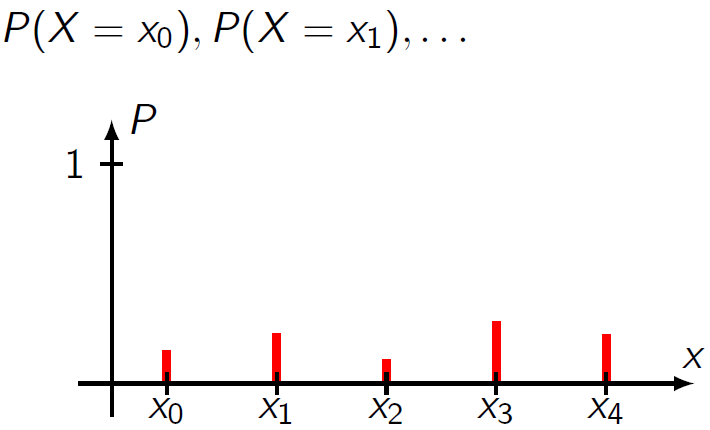
\includegraphics[width=\columnwidth]{images/wahrscheinlichkeit_diskrete_zufallsvariable.png}
\end{minipage}



\subsubsection{Stetige Zufallsvariable}


\begin{minipage}[c]{0.58\columnwidth}
	\raggedright
	Eine Zufallsvariable heisst \textbf{stetig}, wenn sie \textbf{beliebige Werte in einem Intervall} 
	annehmen kann (Wertemenge ist nicht diskret)

	\vspace{0.2cm}

	Beispiel: Messwerte
\end{minipage}
\hfill
\begin{minipage}[c]{0.4\columnwidth}
	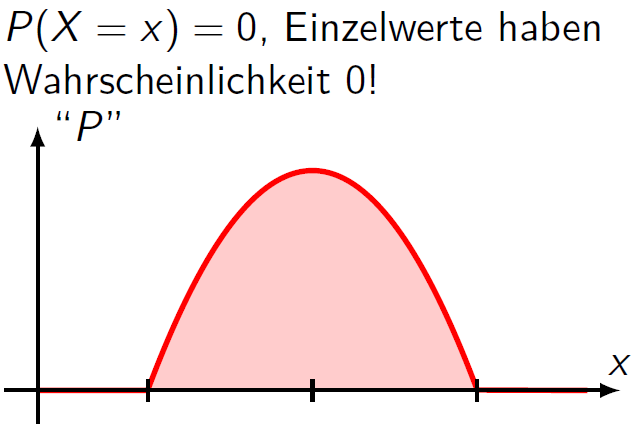
\includegraphics[width=\columnwidth]{images/wahrscheinlichkeit_stetige_zufallsvariable.png}
\end{minipage}




\subsubsection{Notation}

\myul{\textbf{Ereignisse}}

\vspace{0.1cm}

Die Zufallsvariable $X$ definiert neue Ereignisse \\
$A = \{ X \leq a  \} = \{ \omega \in \Omega | X(\omega) \leq a \}$ 

\vspace{0.2cm}

\myul{\textbf{Wahrscheinlichkeiten}}

\vspace{0.1cm}

$P(X \leq a) = P( \{ X \leq a  \}) = P( \{ \omega \in \Omega | X(\omega) \leq a \} )$ 



\subsection[Erwartungswert]{Erwartungswert  $\bm{E(X)}$} 

Il valore atteso $E(X)$ è la media che otterresti ripetendo l'esperimento infinite volte: si calcola sommando ogni valore possibile moltiplicato per la sua probabilità.

$$  \boxed{ E(X) =\sum \text{Wert} \cdot \text{Wahrscheinlichkeit} } $$
$$ E(X) = \sum\limits_{\omega \in \Omega} X(\omega) \cdot P(\{ \omega \} ) = \sum\limits_{i=1}^k X(A_i) \cdot P(A_i)  $$ 
wobei $X$ konstant auf $A_i$ und $\cup \, A_i = \Omega$ sein muss.


\subsection{Empirischer Erwartungswert}

Der Empirische Erwartungswert entspricht einem \textbf{gewichteten Mittelwert} \\
\textrightarrow\ Notenberechnung

\begin{minipage}[c]{0.48\columnwidth}
	$$ P(X = x_i) = \frac{n_i}{n} $$
\end{minipage}
\hfill
\begin{minipage}[c]{0.48\columnwidth}
	\begin{tabular}{ll}
		$n_i$	& Gewichtung 		\\
		$n$ 	& Anzahl Messwerte
	\end{tabular}
\end{minipage}

\vspace{0.2cm}

$$ \boxed{ E(X) = \sum\limits_i X(i) \cdot P(X = x_i) \approx \sum\limits_i x_i \cdot \frac{n_i}{n} = \frac{x_1 n_1 + ... + x_k n_k}{n} } $$


\subsection{Rechenregeln Erwartungswert}

\textbf{Intuition:} Rechenregeln vom Differenzieren / Integrieren funktionieren auch für den Erwartungswert!


\renewcommand{\arraystretch}{1.6}
\begin{tabular}{@{}l l l@{}}
	\textbf{Regel}				& \textbf{Formel}							& \textbf{Bemerkung} \\ \hline
	Konstante als Faktor		& $E(\cor{\lambda} X) = \cor{\lambda} \, E(X)$	& $\lambda$ si porta fuori dalla $\sum$ \\
	Konstante $a$				& $E(a) = a$									& costante: nessuna casualità \\
	EW vom EW					& $E(E(X)) = E(X)$							& $E(X)$ è già una costante \\
	Summe						& $E(X + Y) = E(X) + E(Y)$					& vale \textbf{sempre} \\
	Linearität					& $E(\lambda X + a) = \lambda \, E(X) + a$	& \\
\end{tabular}
\renewcommand{\arraystretch}{1}

\smallskip
{\small \myul{\textbf{Herleitung Summe:}} \;
$E(X + Y) = \sum\limits_{\omega} \big( X(\omega) + Y(\omega) \big) P(\omega) = \sum\limits_{\omega} X(\omega) P(\omega) + \sum\limits_{\omega} Y(\omega) P(\omega)$}

\subsubsection{Verbindung zur Wahrscheinlichkeit}

\textrightarrow\ Es gibt \textbf{nur zwei mögliche Versuchsausgänge}, man gewinnt oder man gewinnt nicht

\vspace{0.2cm}

Ist $ A \subset \Omega$ ein Ereignis, dann ist die \textbf{charakteristische Funktion} $\chi_A$ von $A$ eine Zufallsvariable 
$$ \chi_A: \, \Omega \rightarrow \mathbb{R}: \omega \mapsto \chi_A(\omega) =
\begin{cases} 1 & \omega \in A \\ 0 & \omega \notin A \end{cases} $$
Ihr Erwartungswert ist 
$$ \boxed{ E(\chi_A)= P(A) } $$

\vspace{0.2cm}

\myul{\textbf{Herleitung}}

\vspace{0.1cm}

$ E(\chi_A )=  \chi_A(A) \cdot P(A) + \chi_A(\overline{A}) \cdot P(\overline{A}) = 1 \cdot P(A) + 0 \cdot (1- P(A)) = P(A) $


\subsection{Unabhängigkeit}

$X$ und $Y$ sind unabhängig, wenn die Ereignisse $\{ X \leq x \} $ und $\{ Y \leq y \} $ unabhängig sind.

\vspace{0.2cm}

\begin{minipage}[c]{0.48\columnwidth}
	\begin{center}
		\crd{Bei Unabhängigkeit gilt:}
	\end{center}
	$$ \boxed{ E(XY) = E(X) \cdot E(Y) }$$
\end{minipage}
\hfill
\begin{minipage}[c]{0.48\columnwidth}
	\begin{tabular}{lcl}
		unabhängig		& $\Rightarrow$		& unkorreliert	\\
		unkorreliert 	& $\nRightarrow$ 	& unabhängig
	\end{tabular}
\end{minipage}\vspace{1em}
\begin{itemize}
	\item \textbf{Indipendenti}: conoscere $X$ non dice nulla su $Y$.
	\item \textbf{Scorrelate}: tra $X$ e $Y$ non c'è nessuna tendenza lineare, ma può esserci un legame di altro tipo.
\end{itemize}

Esempio: $X \in \{-1, 0, 1\}$ e $Y = X^2$. $Y$ dipende completamente da $X$ (parabola), ma non c'è nessuna tendenza lineare, quindi sono scorrelate ma dipendenti.

\subsection[Varianz]{Varianz $\bm{\var(X)}$}

Die Varianz misst die 'Streuung' einer Zufallsvariable und entspricht der \textbf{mittleren quadratischen Abweichung vom Erwartungswert.} \\
Die Formel gilt auch für empirische Daten (Messwerte)

\begin{minipage}[c]{0.4\columnwidth}
	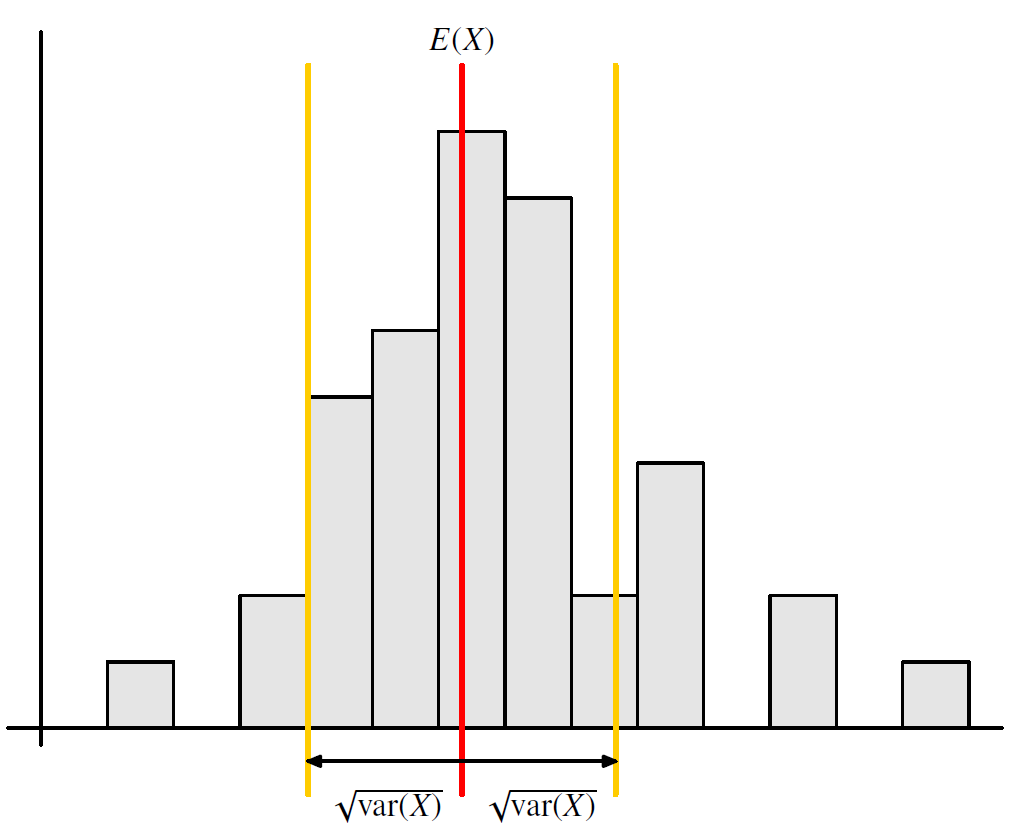
\includegraphics[width=\columnwidth]{images/varianz_darstellung.png}
\end{minipage}
\hfill
\begin{minipage}[c]{0.5\columnwidth}
	\centering
	$$ \boxed{  \var(X) = E( \, (X - E(X))^2 \, ) }  $$
	$$ \boxed{  \var(X) = E(X^2) - E(X)^2 } $$\medskip

	wo $E(X^2) = \sum\limits_{\omega \in \Omega} X(\omega)^2 \cdot P(\{ \omega \})$
\end{minipage}


\subsubsection{Rechenregeln Varianz}

\crd{Für \textbf{unabhängige} Zufallsvariablen} $X$ und $Y$ gilt:

\begin{minipage}[c]{0.48\columnwidth}
	$$ \boxed{  \var(\lambda \, X) = \lambda^{\crd{2}} \var(X) } $$
\end{minipage}
\hfill
\begin{minipage}[c]{0.48\columnwidth}
	$$ \boxed{  \var(X + Y) = \var(X)+ \var(Y) } $$
\end{minipage}


\subsection[Kovazianz]{Kovazianz $\cov(X, \, Y)$}

Die Kovarianz ist ein Korrelationsmass für $X$ und $Y$ 
$$ \boxed{ \cov(X, \, Y) = E(XY) - E(X) \cdot E(Y) } $$

$\operatorname{cov}(X,Y) = 0$ heisst nur: kein \textbf{linearer} Zusammenhang.

\subsection{Tschebyscheff-Ungleichung}

\textbf{Wahrscheinlichkeit, ausserhalb der Toleranz zu landen} \\
Ist $X$ eine Zufallsvariable mit Erwartungswert $\mu = E(X)$, dann gilt:

\vspace{0.2cm}

\begin{minipage}{0.48\columnwidth}
	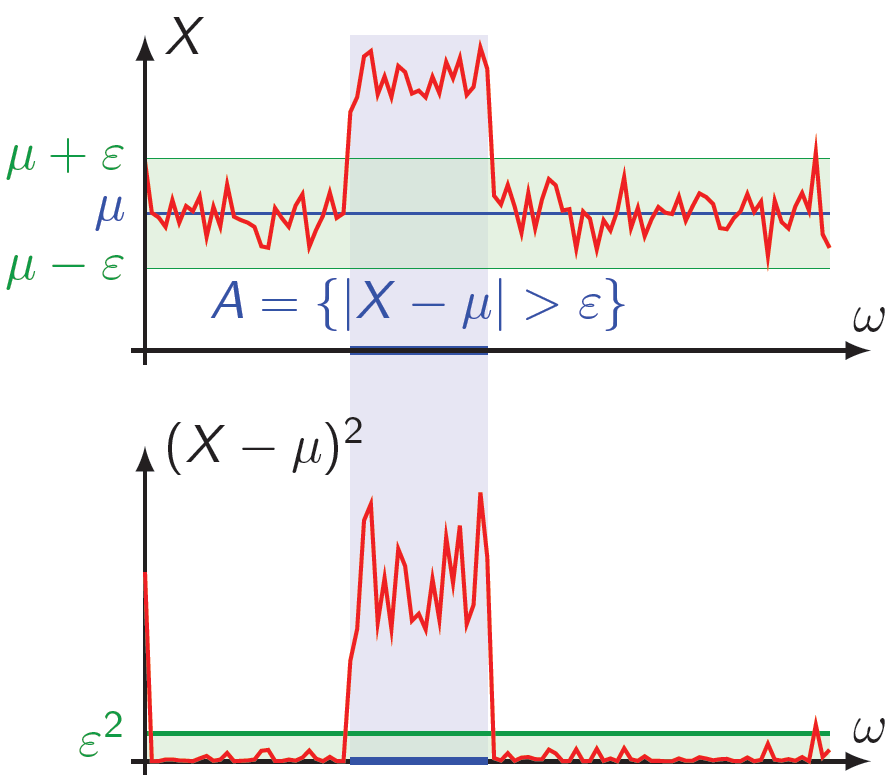
\includegraphics[width=\columnwidth]{images/tschebyscheff_ungleichung.png}
\end{minipage}
\hfill
\begin{minipage}{0.48\columnwidth}
	$$ \boxed{ P( | \crd{X} - \mu | > \varepsilon ) \leq \frac{\var(X)}{\varepsilon^2} = A } $$
	
	\medbreak

	$A$: tutto quello che è fuori da $\mu \pm \varepsilon$\smallbreak

	\textrightarrow\ Wenn die Streubreite (Varianz) zunimmt, nimmt auch die Wahrscheinlichkeit zu, ausserhalb der 'Toleranz' zu landen
\end{minipage}


\subsection{Bernoulli: Genauigkeit des Mittelwertes}

\textbf{Domanda:} quanto può sbagliare la media di $n$ misure rispetto al vero valore $\mu$?

\textbf{Gegeben:} $n$ Messungen $X_1, \ldots, X_n$ (unabhängig), alle mit \\
gleichem Erwartungswert $\mu = E(X_i)$ und gleicher Varianz $\var(X_i) = \var(X)$

\begin{minipage}[c]{0.5\columnwidth}
	\textbf{Mittelwert} (media delle misure):
	$$ M_n = \frac{X_1 + \ldots + X_n}{n} $$
	$$ E(M_n) = \mu \qquad \boxed{ \var(M_n) = \frac{\var(X)}{n} } $$
	\small perché: $\var(\tfrac{1}{n} \sum X_i) = \tfrac{1}{n^2} \cdot n \var(X)$
\end{minipage}
\hfill
\begin{minipage}[c]{0.46\columnwidth}
	\centering
	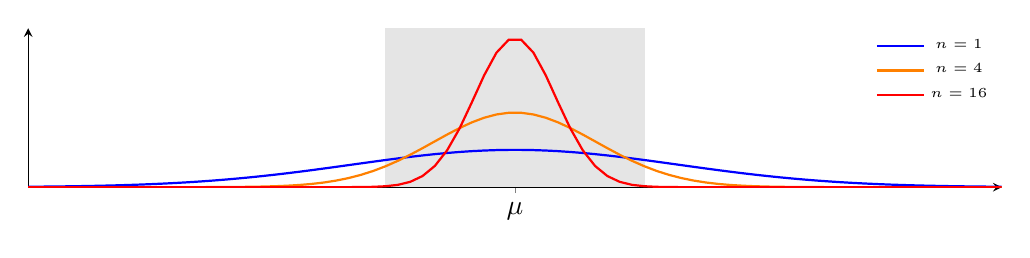
\begin{tikzpicture}
		\begin{axis}[width=1.15\linewidth, height=3.6cm, axis lines=left,
			xtick={0}, xticklabels={$\mu$}, ytick=\empty, ymin=0, ymax=1.7,
			samples=80, domain=-3:3, legend style={font=\tiny, draw=none, at={(1,1)}, anchor=north east}]
			\fill[gray!20] (axis cs:-0.8,0) rectangle (axis cs:0.8,1.7);
			\addplot[thick, blue]   {exp(-x^2/2)/sqrt(2*pi)};
			\addplot[thick, orange] {2*exp(-2*x^2)/sqrt(2*pi)};
			\addplot[thick, red]    {4*exp(-8*x^2)/sqrt(2*pi)};
			\legend{$n=1$, $n=4$, $n=16$}
		\end{axis}
	\end{tikzpicture}
	\\ \tiny distribuzione di $M_n$: più $n$ cresce, più è stretta \\ (zona grigia $= \mu \pm \varepsilon$)
\end{minipage}

\medskip
Tschebyscheff angewendet auf $M_n$ (al posto di $\var(X)$ si mette $\var(M_n)$):
$$ \boxed{ P( | M_n - \mu | > \varepsilon ) \leq \frac{\var(X)}{ n \cdot \varepsilon^2} } $$

\textrightarrow\ Je mehr Messungen, desto unwahrscheinlicher eine grosse Abweichung des Mittelwerts vom Erwartungswert. \\
\textrightarrow\ L'errore tipico (deviazione standard) scende come $1/\sqrt{n}$: per dimezzarlo servono $4\times$ misure.


\subsection{Bernoulli: Gesetz der grossen Zahlen}

\textbf{Domanda:} la frequenza relativa osservata si avvicina alla probabilità vera $P(A)$? \\
\textbf{Idea:} è lo stesso caso di 3.9, con una variabile che vale solo $0$ o $1$.

\begin{tabular}{@{}ll@{}}
	Experiment		& $X = \chi_A = \begin{cases} 1 & A \text{ eingetreten} \\ 0 & \text{sonst} \end{cases}$ \\[0.6em]
	Kennwerte		& $E(X) = P(A)$, \quad $\var(X) = P(A)\,(1-P(A))$ \\[0.3em]
	$n$-mal wiederholt	& $X_1, \ldots, X_n$ \\[0.3em]
	Relative Häufigkeit	& $h_n = \dfrac{X_1 + \ldots + X_n}{n}$ \quad (= quante volte $A$ / $n$) \\[0.6em]
	Kennwerte		& $E(h_n) = P(A)$, \quad $\var(h_n) = \dfrac{P(A)(1-P(A))}{n}$
\end{tabular}

\medskip
Formel aus 3.9 mit $M_n = h_n$, $\mu = P(A)$:
$$ \boxed{ P( | h_n - P(A) | > \varepsilon ) \leq \frac{P(A)(1-P(A))}{ n \cdot \varepsilon^2} \leq \frac{1}{4 \, n \, \varepsilon^2} } $$

\small L'ultima stima vale sempre, perché $P(A)(1-P(A)) \leq \tfrac14$ (massimo per $P(A) = \tfrac12$): utile se $P(A)$ non è noto. \normalsize

\textrightarrow\ Je grösser $n$, desto kleiner die Wahrscheinlichkeit, dass die relative Häufigkeit stark von der Wahrscheinlichkeit abweicht.


\subsection{Lineare Regression (Vorlage!)}

Ein Set von Messwerten $(x, \, y)$ soll mit einer \textbf{Geraden} $y = \cbl{a} \cdot x + \cbl{b}$ \textbf{approximiert} werden. 
Dabei sollen die Parameter $\cbl{a}$ und $\cbl{b}$ der Geraden so bestimmt werden, dass der \textbf{Fehler  $\var(Y-aX-b)$ \\ 
der Approximation minimal} wird.

\vspace{0.2cm}

\textrightarrow\ Entspricht 'Least Squares' Verfahren aus der Linearen Algebra 

$$  \boxed{ \cbl{a} = \frac{E(XY) - E(X) E(Y)}{E(X^2) - E(X)^2} = \frac{\cov(X,Y)}{\var(X)} } $$
$$  \boxed{ \cbl{b} = E(Y) - \cbl{a}  E(X) } $$


\subsubsection{Fehlerberechnung der Approximation}

\myul{\textbf{Fehler $\bm{Z}$}}
$$ \boxed{ Z = \var(Y) \Big( 1 - \frac{\cov(X,Y)^2}{\var(X) \, \var(Y)} \Big) = \var(Y)(1-r^2) } $$ 

\vspace{0.2cm}

\myul{\textbf{Regressionskoeffizient $r$}}
$$ \boxed{ r = \frac{\cov(X, Y)}{\sqrt{\var(X) \cdot \var(Y)}} } $$

\textrightarrow\ Der Fehler $Z$ wird klein, wenn $r^2$ nahe bei $1$ ist, also $r$ nahe bei $\pm 1$


\subsection{Nichtlineare Regression}

Mit einigen 'Umwandlungs-Tricks' können auch einige nichtlineare Funktionen linear gemacht werden und somit wieder
linear approximiert werden

\begin{center}
	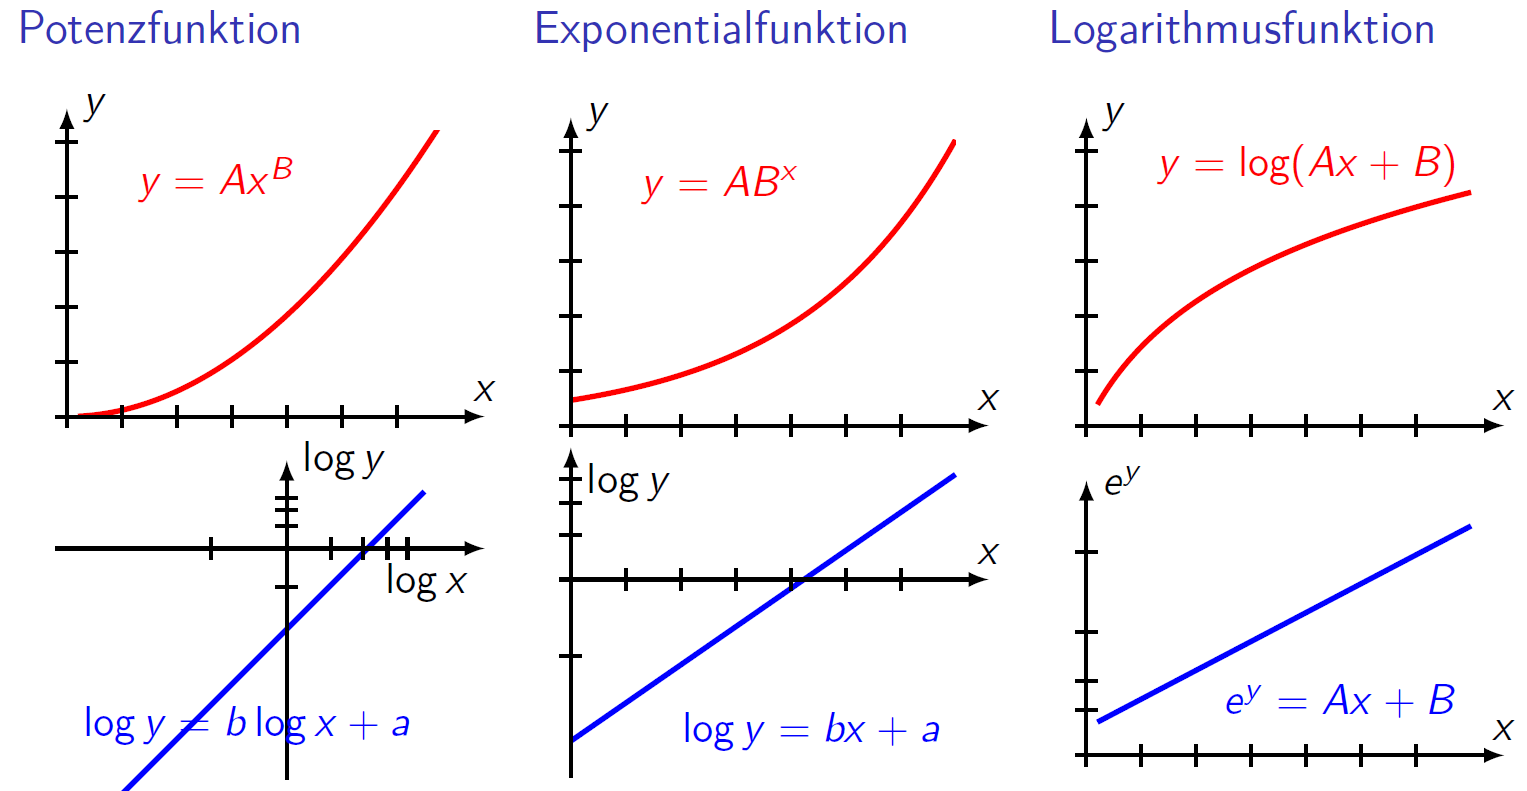
\includegraphics[width=0.8\columnwidth]{images/nichtlineare_regression.png}
\end{center}

\begin{tabular}{l c l}
	$y = Ax^B$			& \textrightarrow\	& $\log(y) = b \log(x) + \log(a)$ 	\\
						& \textrightarrow\ 	& $X = \log(x)$ ; $Y = \log(y)$ 	\\
	\\	
	$y = AB^x$ 			& \textrightarrow\ 	& $\log(y) = x (\log(B)) + \log(A)$ \\
						& \textrightarrow\ 	& $X = x$ ; $Y = \log(y)$ 			\\
	\\		
	$y = \log(Ax +B)$ 	& \textrightarrow\ 	& $e^y = Ax + B $					\\
						& \textrightarrow\ 	& $X = x$ ; $Y = e^y$
\end{tabular}

